The neat thing about a process network is that you can swap one process for another if it ``speaks the same language.'' By this, we mean that you can swap one process for another if the input channels and the output channels carry the same kind (or type) of information. 

In this short chapter, we'll make one change to the code from \nameref{ch4} to demonstrate this. 

\section{Seeing the parts}
We just finished writing our first process network; now, lets tear it apart. This network was made up of two processes, \bp and \tp. 

\begin{figure}[ht]
  \begin{center}
    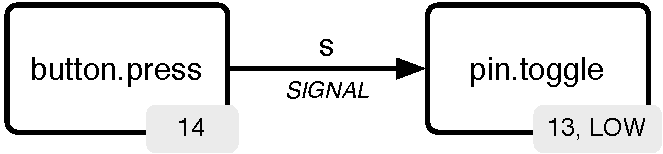
\includegraphics[width=0.8\linewidth]{images/ch4-button-toggle-led}
    \caption{Our two-process network.}
    \label{diagram:ch4-button-toggle-led-also-wik}
  \end{center}
\end{figure}

\newpage

If we look at this process network from the point of view of \bp, we might say:

\begin{quote}
	\bp has one {\strong output} channel, {\code s}, that carries information of type \SIGNALT.
\end{quote}

We can also look at this network from the point of view of \tp. Then, we might say:

\begin{quote}
	\bp has one {\strong input} channel, {\code s}, that carries information of type \SIGNALT.
\end{quote}

\begin{figure}
\begin{center}
\subfigure[One output channel...] % caption for subfigure a
{
    \label{diagram:ch5a-button-press-only}
    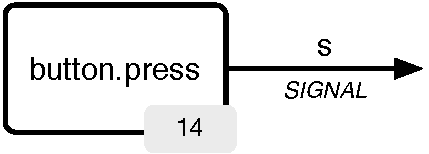
\includegraphics[width=4cm]{images/ch5a-button-press-only}
}
\hspace{1cm}
\subfigure[... or one input channel.] % caption for subfigure b
{
    \label{diagram:ch5a-pin-toggle-only}
    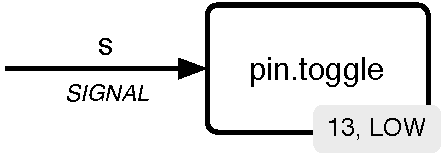
\includegraphics[width=4cm]{images/ch5a-pin-toggle-only}
}
\caption{}
\label{diagram:button-and-pin} % caption for the whole figure
\end{center}
\end{figure}

We can see these two ways of looking at the parts of our process network in Figure~\ref{diagram:button-and-pin}. Now we'll introduce a new new \PROCedure from the \plumbing library: {\code tick}.

\begin{figure}[!h]
  \begin{center}
    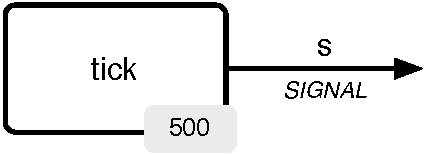
\includegraphics[width=0.6\linewidth]{images/ch5-tick}
    \caption{Another \PROCedure in the \plumbing library.}
    %\label{diagram:ch4-button-toggle-led-also-wik}
  \end{center}
\end{figure}

\newpage

The process {\code tick} takes two parameters: the first is the number of milliseconds between ticks, and the second is the sending end of a channel that carries signals. Now, here's the code from Chapter~\ref{ch4}:

\vspace{3mm}
\lstinputlisting[caption=Our original program uses {\code button.press}.]{code/button-toggle-led.occ}

Because both \bp and {\code tick} have the same inputs (none) and the same outputs (one channel that carries messages of type \SIGNALT), we can substitute one for the other. Once we do that substitution, our code looks like:

\vspace{3mm}
\lstinputlisting[caption=One substitution changes the program.]{code/tick-toggle-led.occ}

Because the \tp process expects a \SIGNALV to tell it when to turn its pin on or off, it doesn't matter where that signal comes from. It could be that it comes from a button press, or it could come from a clockwork ticker! 

\newpage

\section{Exploring ``plug-n-play''}
As we continue to explore the \plumbing library, you are encouraged to experiment with modifications of your existing process network. Particularly, we hope you explore this notion of what we call ``plug-n-play.'' 

Process networks are connected by {\CHANnel}s. As you saw in this chapter, we can get very different behavior from very similar code, simply by replacing one process with another. When using \occam and the \plumbing library, your should strive to write lots of small, simple {\PROCedure}s. Then, you can combine these {\PROCedure}s into a process network, and (most importantly) rearrange the process network (or substitute one process for another) if you want to get different behavior from your program. 

\begin{wrapfigure}{r}{0.5\linewidth}
		\vspace{-8mm}
	  \begin{center}
    	
\includegraphics[width=0.9\linewidth]{images/matthews-runaway-small}
		  \captionsetup{labelformat=empty, font=footnotesize}
			\caption{{\em Matthew's Runaway} was a piece of art developed by substituting one {\PROCedure} for another.}
    	%\label{screenshot:compile-successful}
  \end{center}
\end{wrapfigure}

For example, if you are developing a piece of art that you intend to be interactive, you might start by testing it with a process like {\code tick}. Then, when you're done programming, you might switch that with a process that handles input from the world (eg. \bp). Then, your piece is ready for interaction with people viewing your piece in a gallery.